\documentclass{article}
\setlength{\parskip}{5pt} % esp. entre parrafos
\setlength{\parindent}{0pt} % esp. al inicio de un parrafo
\usepackage{amsmath} % mates
\usepackage[sort&compress,numbers]{natbib} % referencias
\usepackage{url} % que las URLs se vean lindos
\usepackage[top=25mm,left=20mm,right=20mm,bottom=25mm]{geometry} % margenes
\usepackage{hyperref} % ligas de URLs
\usepackage{graphicx} % poner figuras
\usepackage[spanish]{babel} % otros idiomas
\usepackage[utf8]{inputenc}
\author{Brenda Giselle Hinojosa \\ Armando Rincon Reyes \\ Cynthia Belén Guerrero Pardo \\ Juan Jose Prado Luna \\ Luis Fernando Martinez Ovalle} % author
\title{Tarea 1} % titulo
\date{\today}

\begin{document} % inicia contenido

\maketitle % cabecera

\begin{abstract} % resumen
Este documento es la investigación de los elementos más básicos que estructuran la biomecánica para poder entender este tema desde cero y dar una breve introducción al lector de lo que conlleva. La idea del concepto de biomecánica no es la misma que todos tenemos, lo mismo pasa con el objetivo que esta tiene. Por eso, la definición de biomecánica, los propósitos que esta tiene, entre otros aspectos serán los que tomaremos principalmente en cuenta para poder resumir de la mejor manera esta investigación y que todos tengamos el mismo entendimiento de esta ingeniería.
\end{abstract}


\section{Introducci\'{o}n}\label{intro} % seccion y etiqueta
En el presente reporte estaremos hablando sobre la biomecánica, con el objetivo de realizar una investigación y profundizar en los temas más importantes que pueden abarcar esta materia para conseguir una introducción lo más completa posible del tema mencionado. La definición de la mecánica, cinética, movimiento y otros conceptos importantes serán clave para el entendimiento completo de lo que puede llegar a involucrar la biomecánica. 
De igual manera, todo lo investigado nos hará tener una mejor idea de los objetivos y los beneficios que trae este tema consigo. Disminuir las lesiones, mejorar el aguante de articulaciones, son solo unos dos los beneficios que implica la biomecánica. Además, la biomecánica es una ingeniería que envuelve otras ingenierías, el estudio y la práctica de esta no se puede realizar sin antes haber contemplado las nociones de otras ingenierías.  


\section{Desarrollo}

\cite{ff4}\textbf{¿Qué es la biomecanica?} \\
“La biomecánica es una rama de la cinesiología, la cual se dedica principalmente al estudio del movimiento humano desde el punto de vista de las ciencias físicas.” \\ \\
\textbf{¿Por qué es importante la biomecánica?} \\
Esta nos ayuda a analizar y evaluar las destrezas y capacidades motrices, de manera que se aplique de forma eficiente una técnica o una adaptación buscando la mayor capacidad y rendimiento deportivo. \\ \\
\textbf{¿Cuáles son los objetivos a tener en cuenta?}
\begin{description}
\item •	Analizar actividad o gesto deportivo y observar desequilibrios musculares que intervienen y tienen importancia en una actividad concreta o en el desarrollo de una capacidad.
\item •	Valorar y medir de forma cualitativa los movimientos directamente relacionados con la práctica deportiva.
\item •	Con esto, determinar y corregir los defectos de actuación deportiva y por tanto adaptar técnicas apropiadas para el correcto desarrollo y éxito deportivo.
\item •	Determinar factores de riesgo de lesión. 
\end{description}
\textbf{Conceptos de la física dentro de la biomecánica} \\
Dentro de la biomecánica, encontramos los conceptos de cinética (estudio de las fuerzas que actúan sobre el cuerpo) y cinemática (estudio de los movimientos del cuerpo). Cinco importantes componentes de la biomecánica son el movimiento, la fuerza, el momento, las palancas y el equilibrio: 
\begin{description}
\item[Movimiento]:hace referencia al desplazamiento del cuerpo o de un objeto a través del espacio. La velocidad y la aceleración son componentes importantes del movimiento.
\item[Fuerza]:hace referencia al empuje o la tracción que provocan que una persona o un objeto aceleren, reduzcan la velocidad, se detengan o cambien de dirección.
\item[Momento]:hace referencia al resultado de una masa y de su velocidad en su desplazamiento.
\item[Palancas]:nuestros brazos y piernas funcionan a modo de palancas; una palanca está formada por tres componentes: el brazo de resistencia, el punto de apoyo y el eje de rotación.
\item[Equilibrio]:hace referencia a la estabilidad. Un principio importante del equilibrio es la alineación del centro de gravedad del cuerpo sobre la base de apoyo. Tener un buen equilibrio es importante para la práctica de muchos deportes y ejercicios.
\end{description} 
\begin{figure} [htp]% figura
    \centering
    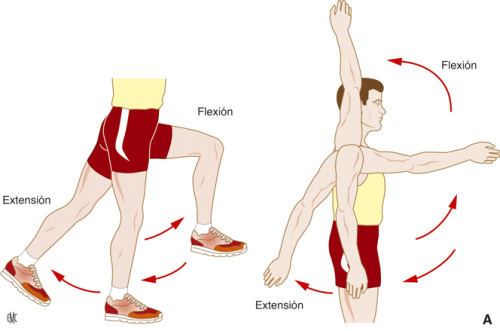
\includegraphics[width=150mm]{representacion biomecanica.jpg} % archivo
    \caption{Representación de la Biomecánica}
    \label{grafica}
\end{figure}
\textbf{Relación de la mecánica con la biomecánica} \\
La mecánica es el área de la física que se ocupa del estudio del movimiento de objetos macroscópicos. Las distintas fuerzas que pueden aplicarse a los objetos resultan en desplazamientos o cambios en la posición de un objeto. Las descripciones modernas del movimiento comienzan con una definición cuidadosa de magnitudes como el desplazamiento, el tiempo, la velocidad, la aceleración, la masa y la fuerza. \cite{ff3}
\begin{description}
\item •	La mecánica clásica: Es la disciplina que estudia el movimiento de los objetos ordinarios de la Tierra, centrada en objetos cuya velocidad es menor que la velocidad de la luz. Está basada en la mecánica newtoniana y posee como elementos centrales la gravedad, la masa y el movimiento.
\item •	La mecánica relativista:  Describe el comportamiento de cuerpos que se mueven a grandes velocidades en el espacio y el tiempo, como los cuerpos celestes. Está relacionada con la teoría de la relatividad de Albert Einstein.
\item •	La mecánica cuántica: Enfocada al estudio de los fenómenos que ocurren a nivel microscópico, analizando el comportamiento y la radiación electromagnética de la materia, pero a una escala atómica y subatómica.
\item •	La teoría cuántica de campos: Esta teoría consigue asociar los principios cuánticos y la teoría de la relatividad especial. Su principal aplicación es la física de altas energías, para estudiar las partículas subatómicas.
\end{description}
\begin{figure} [htp]% figura
    \centering
    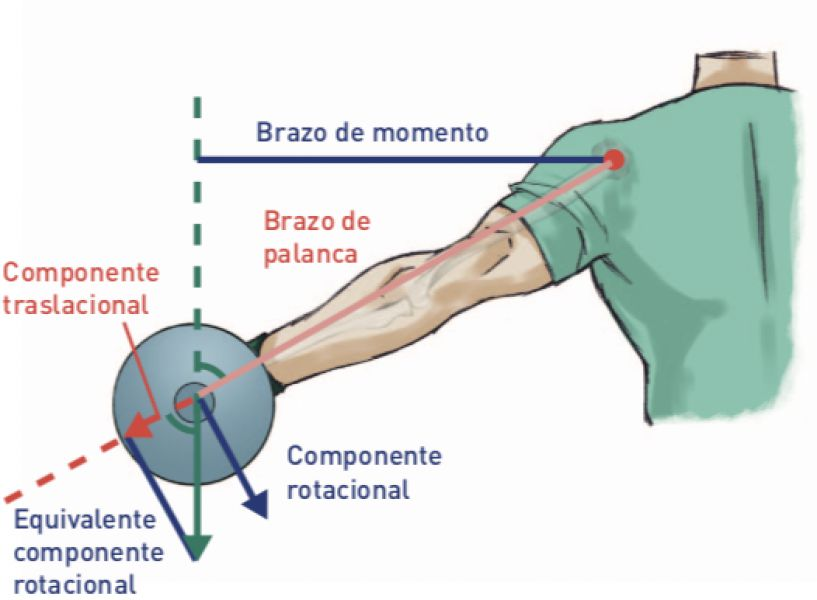
\includegraphics[width=100mm]{mecanica biomecanica.jpg} % archivo
    \caption{Mecánica y Biomecánica}
    \label{grafica}
\end{figure}
\textbf{Aplicaciones de la Biomecánica} \\
La Ingeniería Biomecánica se ubica a mitad de camino entre la Biología y la ingeniería Mecánica e incluso la Medicina. La Mecánica tiene aplicaciones en el campo de la Biología y viceversa, lo que es necesario para la comprensión de esta disciplina. \\
Actualmente, existen grandes avances en tecnología, que pueden ser muy beneficiosos en tratamientos relacionados con la salud para mejorar la calidad de vida. Aquí, la Ingeniería Biomecánica se aplica a diversas disciplinas médicas, surgiendo lo que conocemos como biomecánica médica. \\
En este caso se investiga el ámbito de la biomecánica del movimiento humano, más concretamente acerca del análisis y simulación dinámica del movimiento, así como en el diseño de dispositivos robóticos de rehabilitación para personas con movilidad reducida. Se desarrollan tecnologías aplicables, por ejemplo, en la industria ortopédica y del calzado, en centros hospitalarios, y en centros de alto rendimiento deportivo. \cite{ff2} \\
En la actualidad, es muy común ver trabajos de ingeniería relacionados con las siguientes áreas:\cite{ff2}
\begin{enumerate}
    \item Captura, análisis y simulación dinámica del movimiento humano. Análisis de la marcha de personas sanas y de la marcha patológica.
    \item Desarrollo de modelos multicuerpo antropométricos para el análisis dinámico y el cálculo de fuerzas musculares durante el movimiento.
    \item Simulación y diseño de dispositivos robóticos de rehabilitación para personas con movilidad reducida. Entre ellos, ortesis activas para asistencia de personas con lesión medular.
    \item Predicción de fuerzas de contacto en las articulaciones del cuerpo humano mediante técnicas no invasivas.
    \item Análisis de distintos aspectos relacionados con el confort del calzado.
    \item Aplicación del análisis del movimiento humano en el deporte.
\end{enumerate}
La Ingeniería Biomecánica también relaciona la biología de los seres humanos con la mecánica de ingeniería, surgiendo así la biomecánica industrial. Un Perito en el área puede estudiar cómo reacciona el cuerpo humano ante, por ejemplo, en un accidente automovilístico (o de cualquier otra índole). Así como analizar si las medidas de seguridad en posibles accidentes de tráfico son suficientes o incluyo perjudiciales. \cite{ff1} \\
Mediante la evaluación de los accidentes en el contexto de este tipo de ingeniería, pueden mejorar las medidas de seguridad tanto para conductores y pasajeros.\\
Por lo tanto, existen Ingenieros Biomecánicos trabajando en la reconstrucción de accidentes, lo que les permite aplicar los principios de ingeniería en la evaluación de factores humanos, análisis de fallos, e incluso la evaluación de las pruebas basadas en la lesión, todo lo cual es relevante en el caso durante un proceso judicial. \cite{ff1}
\begin{figure} [htp]% figura
    \centering
    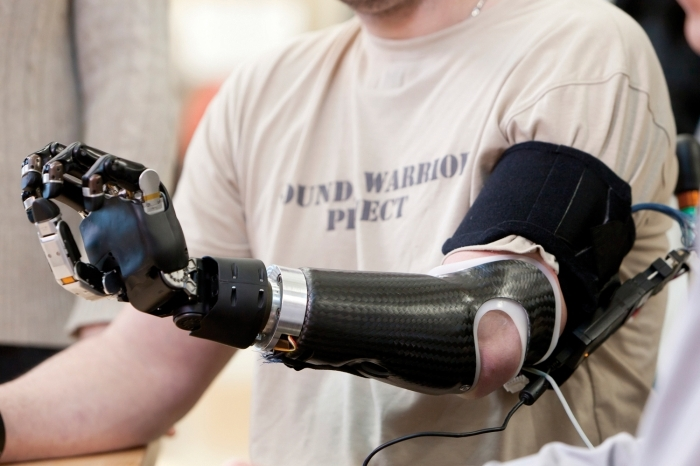
\includegraphics[width=150mm]{aplicacion biomecanica.jpg} % archivo
    \caption{Ejemplo de la aplicación de la Biomecánica}
    \label{grafica}
\end{figure}

\textbf{Beneficios de la biomecánica adecuada} \\
La comprensión de los movimientos adecuados permitirá ser más eficiente, además de desarrollar buenos hábitos posturales a largo plazo. Una persona que incorpora una biomecánica adecuada en sus movimientos corporales reducirá considerablemente el riesgo de lesionarse. \cite{ff5} \\
Ahora veamos algunos de los beneficios de tener una biomecánica adecuada:
\begin{description}
\item •	Desarrolla patrones de movimiento eficientes.
\item •	Minimizar las lesiones.
\item •	Desarrolla hábitos posturales adecuados.
\item •	Conservación de energía a través de la economía del movimiento.
\item •	Ayuda a eliminar los desequilibrios musculares.
\item •	Reduce el desgaste en las articulaciones y los ligamentos.
\item •	En deportistas mejora la forma y el gesto técnico específico del deporte en cuestión.
\end{description}
Todo esto debido a que los músculos generan fuerzas de tracción y aplican movimientos en las articulaciones a través de palancas para proporcionar estabilidad en el cuerpo. Por lo tanto, cualquier lesión de cualquiera de los elementos individuales del sistema musculoesquelético cambiará la interacción mecánica y causará degeneración e inestabilidad en los movimientos.

\section{Conclusiones}

Como ya se mencionó, la biomecánica estudia la mecánica de los organismos vivos, es una ciencia básica y aplicada, que abarca la investigación y el uso práctico de sus hallazgos. La biomecánica, además, incluye cómo los músculos, huesos, tendones y los ligamentos trabajan juntos para producir movimiento. Si es enfocada hacia la kinesiología o cinesiología, centrándose específicamente en la mecánica del movimiento del cuerpo humano, podemos obtener avances tecnológicos que nos permitan mejorar nuestra salud o la calidad de vida en personas con alguna discapacidad motriz, visual o auditiva. \\
En el caso del movimiento corporal humano, el cual se logra mediante una interacción mecánica compleja y altamente coordinada entre los huesos, músculos, ligamentos y articulaciones dentro del sistema musculoesquelético bajo el control del sistema nervioso, la biomecánica juega un papel elemental. Su objetivo principal será comprender la función de todos los mecanismos del sistema musculoesquelético al momento de ejecutar algún movimiento o tarea. Por lo tanto, comprender la biomecánica y la carga de cada elemento que interviene en la misma será de gran beneficio para analizar movimientos, comprender técnicas, gestos deportivos, estudiar las causas de una enfermedad, prevenir posicionamientos y posturas indebidas, entre otras muchas otras. 


\bibliography{bib}
\bibliographystyle{plainnat}

\end{document}
